\scanpage{207}
\uline{Faisons varier} $x$ pt complexe (ou place archimédienne). Je pense que \uline{les} $\xi_{x,\mathbf Z}$ \uline{et même les} $\xi_{x,\mathbf R}$ \inserted{[$\simeq\xi_{x,\mathbf C}$ muni de $\tau$]} \uline{pris respectivement à des places distinctes sont non isomorphes}.

\margin{\figure{\begin{tikzpicture}\node[draw,ellipse,rotate=15,align=center,inner sep=9pt] {faux, cf\\ groupoïde\\ fondamental\\ sur $\mathbf Z$};\end{tikzpicture}}}

Quant aux $\xi_{x,\mathbf C}=\xi_{x,\infty}$, \unsure{eux} \deleted{\unsure{avec}} \inserted{comme} $\unsure{k}$ est \deleted{\unsure{nous avons dit, ils sont}} alg. clos ils sont isomorphes entre eux, mais pas canoniquement ....

\uline{NB} En car $p>0$, je pense que $T_\alpha(\mathbf R)=\varnothing$ pour $\alpha$ grand, ce qui explique qu'il n'y ait pas de phénomènes de ``conjugaison complexe'' ``Ramification en $\mathbf R$'' ... à considérer alors ....

\margin{Vérifier s'il ne peut y avoir des pt à val. dans une \unsure{ext. tot.} réelle ???}

Si

\figure{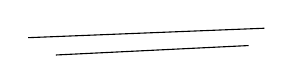
\begin{tikzpicture}\draw (0,0)--(3.0,0.12);\draw (0.35,-0.22)--(2.8,-0.1);\end{tikzpicture}}

Pt motivique de $X$ à valeurs dans un corps (ou un anneau) $h$ : objets de $T(h)$. Langage de la \uline{fibre d'un motif en un point}. Les pts forment une catégorie fibrée sur $(\mathrm{Sch})$ muni de fpqc, \deleted{\illegible{1}} c'est un \uline{torseur}. Pour $h$ donné, les isom. d'un \deleted{objet} $\xi\in T(h)$ sur un autre forment \unsure{le}

\mspage{206}
